%%
%% This is file `sample-authordraft.tex',
%% generated with the docstrip utility.
%%
%% The original source files were:
%%
%% samples.dtx  (with options: `authordraft')
%% 
%% IMPORTANT NOTICE:
%% 
%% For the copyright see the source file.
%% 
%% Any modified versions of this file must be renamed
%% with new filenames distinct from sample-authordraft.tex.
%% 
%% For distribution of the original source see the terms
%% for copying and modification in the file samples.dtx.
%% 
%% This generated file may be distributed as long as the
%% original source files, as listed above, are part of the
%% same distribution. (The sources need not necessarily be
%% in the same archive or directory.)
%%
%% The first command in your LaTeX source must be the \documentclass command.
\documentclass[sigconf,authordraft]{acmart}

%%
%% \BibTeX command to typeset BibTeX logo in the docs
\AtBeginDocument{%
  \providecommand\BibTeX{{%
    \normalfont B\kern-0.5em{\scshape i\kern-0.25em b}\kern-0.8em\TeX}}}

%% Rights management information.  This information is sent to you
%% when you complete the rights form.  These commands have SAMPLE
%% values in them; it is your responsibility as an author to replace
%% the commands and values with those provided to you when you
%% complete the rights form.

\setcopyright{}
\copyrightyear{}
\acmYear{2019}
\acmDOI{}

\usepackage{enumitem}% http://ctan.org/pkg/enumitem

%% These commands are for a PROCEEDINGS abstract or paper.
% \acmConference[Woodstock '18]{Woodstock '18: ACM Symposium on Neural
%   Gaze Detection}{June 03--05, 2018}{Woodstock, NY}
% \acmBooktitle{Woodstock '18: ACM Symposium on Neural Gaze Detection,
%   June 03--05, 2018, Woodstock, NY}
% \acmPrice{15.00}
% \acmISBN{978-1-4503-9999-9/18/06}


%%
%% Submission ID.
%% Use this when submitting an article to a sponsored event. You'll
%% receive a unique submission ID from the organizers
%% of the event, and this ID should be used as the parameter to this command.
%%\acmSubmissionID{123-A56-BU3}

%%
%% The majority of ACM publications use numbered citations and
%% references.  The command \citestyle{authoryear} switches to the
%% "author year" style.
%%
%% If you are preparing content for an event
%% sponsored by ACM SIGGRAPH, you must use the "author year" style of
%% citations and references.
%% Uncommenting
%% the next command will enable that style.
%%\citestyle{acmauthoryear}

%%
%% end of the preamble, start of the body of the document source.
\begin{document}

%%
%% The "title" command has an optional parameter,
%% allowing the author to define a "short title" to be used in page headers.
\title[An Evaluation of Multi-Criteria Recommendation Techniques]{An Evaluation of Multi-Criteria Recommendation Techniques}

%%
%% The "author" command and its associated commands are used to define
%% the authors and their affiliations.
%% Of note is the shared affiliation of the first two authors, and the
%% "authornote" and "authornotemark" commands
%% used to denote shared contribution to the research.

\author{Ariel Martínez Silberstein}
\email{amartinez5@uc.cl}
\affiliation{%
  \institution{Pontifical Catholic University of Chile}
  \city{Santiago}
  \state{Chile}
}

%%
%% By default, the full list of authors will be used in the page
%% headers. Often, this list is too long, and will overlap
%% other information printed in the page headers. This command allows
%% the author to define a more concise list
%% of authors' names for this purpose.
\renewcommand{\shortauthors}{A. Martínez}

%%
%% The abstract is a short summary of the work to be presented in the
%% article.
\begin{abstract}
Although multi-criteria rating systems —in which the rating is composed of a vector along several criteria— are being commonly employed in the industry, recommendation systems that use them correspond to a largely unexplored area. Several reviews show that multi-criteria ratings can be leveraged to produce better personalized recommendations, as compared to traditional techniques. However, much additional work is needed to make significant improvements. To this end, in this paper, we empirically test out two different multi-criteria recommendation models (one that aggreates similarities and another that aggregates ratings) in order to evaluate their rating estimation performance. Our results do not conclude any improvement. Nevertheless, they can be considered as one more step towards the science of understanding the underlying value of multi-criteria ratings.
\end{abstract}


%%
%% Keywords. The author(s) should pick words that accurately describe
%% the work being presented. Separate the keywords with commas.
\keywords{recommender systems, personalized recommendations, multi-criteria ratings, rating prediction}


%%
%% This command processes the author and affiliation and title
%% information and builds the first part of the formatted document.
\maketitle

\section{Introduction}

As rational beings, we attempt to optimize our decision making by searching for the largest amount of information. The problem we have been facing in the last few decades is that the information available to us has significantly increased into an untraceable amount, especially due to the relatively new internet. This increase in information has lead to many intelligent inventions that help us go through the process of decision making, such as recommendation systems, which usually provide users of a certain community with a group of items that are probably relevant to them. Many times, these systems assume that there is a sparse function $R$ that maps every user-item pair into a numerical rating value.

Recommendation systems are typically classified in a few ways. One possible classification is based on their algorithmic nature and separates recommendation systems into \textit{memory-based} (sometimes also referred to as \textit{heuristic-based}) and \textit{model-based} approaches (Adomavicius \& Tuzhilin, 2005). The former can be understood as a recommendation process that occurs on the spot, whilst the latter makes recommendations computed by a predictive architecture, which frequently corresponds to some sort of statistical or machine-learning model. Another classification, as first stated by Balabanovic \& Shoham (1997), focuses on the information the that recommendation system uses to make it's predictions, famously known as \textit{content-based}, \textit{collaborative filtering} and \textit{hybrid} approaches.

Recommendation systems can be further classified into \textit{single-criterion} and \textit{multi-criteria}, depending on the number of numerical ratings they use for each user-item relation. Note that the vast majority of recommendation systems fall into the former, by using a single rating to represent an overall score, turning the multiple criteria systems into a largely unexplored territory, according to Adomavicius \& Kwon (2007). While traditional single-criterion recommendation systems have done well in many domains and applications, several recent works have considered them to be limited in terms of accuracy. With a multi-criteria setting, users are able to express their opinion on more than one attribute of an item, which may lead to better recommendations (Adomavicius et. al., 2011).

The remainder of this paper is structured as follows. In section 2, we briefly review related work that might be of interest to the reader. In section 3, we present a similarity aggregation approach that extends standard collaborative filtering methods into a multi-criteria setting (and thus can be further used in any collaborative filtering context), and a rating aggregation approach, that can be used as a complement to any recommendation technique in order to adapt to a multi-criteria setting. In section 4, we discuss the methodology and database used in this work, followed by a discussion of the results reported by the proposed models contrasted against some selected baselines for a set of experiments. Finally, we conclude this paper in section 5.

\section{Related Work}

Statnikov \& Matusov (1995) first described the majority of engineering issues as multi-criteria optimization problems. However, as Adomavicius et. al. (2011) explain, the solutions to these problems are typically designed to find the items that are optimal in general (\textit{i.e.} with respect to all users in the database), but are unable to compute personalized recommendations. Roy (1996) proposes four steps in order to correctly address and analyze these kind of problems: define the set of alternatives (\textit{i.e.} items) upon a recommendation decision has to be made; identify the functions that declare the preferences of the user for each criterion; specify a \textit{global preference model} (the function that synthesises the user's partial preferences into an overall utility); and design a concrete procedure or methodology for the decision making process.

Traditional similarity metrics such as the Pearson Correlation or the Cosine-based only consider a single rating. Therefore, in order to take into account a multiple rating setting, these expressions must be either tweaked accordingly, aggregated or completely replaced. Adomavicius \& Kwon (2007) introduce the \textit{average} (by averaging all individual similarities) and \textit{worst-case} (by using the smallest similarity) aggregation approaches. Tang \& McCalla (2009) propose a \textit{weighted sum} of the similarities, in which the weights represent the importance of each individual rating. In other works, it is preferred to simply employ the inverse of a multidimensional distance metric such as the Manhattan, Euclidean or Chebyshev, where each dimension corresponds to one of the individual criteria. Note that all of these techniques can be used in combination with any traditional recommendation scenario, because their result is a single (may be called overall) rating score.

On the other hand, some works propose novel model-based recommendation systems that leverage the information contained in multi-criteria rating settings. Sahoo et. al. (2006) developed a tree-based probabilistic model for estimating an overall score. Li et. al (2008) propose a \textit{multilinear singular value decomposition} (MSVD) approach, which extends the traditional SVD thechnique. They show that MSVD can be used to find non-trivial relationships between users, items and rating criteria. Other papers engage the multi-criteria rating issue during the recommendation process, such as Manouselis \& Costopoulou (2007), that designed a method for calculating the total utility of a given user-item pair through an aggregate function that computes a weighted sum of all the individual criterion utilities.

Multi-criteria recommendation has been studied in the past, but it's still vastly unexplored and there has not been much progress in the area during the last decade. As a matter of fact, Nilashi et. al. (2014) is one of the newest important works on the topic, in which they propose a hybrid approach for multi-criteria collaborative filtering settings. It would be fair to say that most contributions were made a long time ago. Hence, a more comprehensive research literature survey can be found in Adomavicius et. al. (2011).

\section{The Models}

In this section, we describe two multi-criteria recommendation frameworks to be tested in this paper, illustrated in Figure~\ref{fig:diagram}.

\begin{figure*}[h]
  \centering
  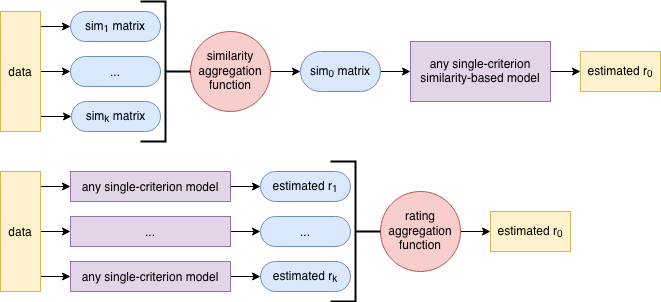
\includegraphics[scale=0.5]{static/diagram.png}
  \caption{The similarity aggregation (section~\ref{sec:similarities}) and rating aggregation (section~\ref{sec:ratings}) frameworks, respectively.}
  \label{fig:diagram}
\end{figure*}

\subsection{Aggregating Similarities}
\label{sec:similarities}

Adomavicius \& Kwon (2007) propose two ways of aggregating traditional similarities based on individual ratings. These approaches can use any similarity metric, such as the Cosine-based or the Pearson Correlation (here, we use the former). Let us assume that each rating given by user $u$ to item $i$ is constructed by $k + 1$ individual ratings $r_0, ..., r_k$, where $r_0$ is an overall rating and the rest correspond to specific ones. This is useful, because multi-criteria rating systems provide relevant information that can be leveraged to make better rating predictions. The following example shows how.

In the standard collaborative filtering approach, a recommendation system usually attempts to find the nearest neighbors of a given user or item. Consider the former, in which we wish to predict the rating user $u$ would give to item $i$. The nearest neighbors of $u$ would have to be other users who have consumed $i$ and have qualified other items similarly to $u$. Further consider that both users $u$ and $u^\prime$ have consumed item $i^\prime$ and given it a rating value of $3$, \textit{i.e.},

\begin{align}
    R(u, i^\prime) = R(u^\prime, i^\prime) = 3
\end{align}

One could say that those users are similar because the ratings they gave are the same. Nonetheless, let us shift to a multi-criteria scenario, in which, for simplicity, the rating system consists of $3$ scalars ($1$ overall and $2$ specific) and the rating values given are the following.

\begin{align}
    R(u, i^\prime) = (4, 1, 5) \\
    R(u^\prime, i^\prime) = (4, 5, 1)
\end{align}

In the example above, both overall ratings are the same. However, it is clear to see that the user's tastes and opinions are opposites, given the nature of the specific ratings. This is one way of understanding the underlying information contained in multi-criteria ratings, which can be leveraged to better compute KNN algorithms.

The overall similarity is then proposed to be calculated in one of the following ways, where $sim_i (u, u^\prime)$ is the similarity between $u$ and $u^\prime$ based on the $i$-th criterion ($r_i$): the \textit{average} (equation 4) and \textit{worst-case} (equation 5) similarities. The former is computed by averaging all individual similarities, whilst the latter does it by taking the smallest of all individual similarities. Similarly, one can construct an additional aggregation function by taking the \textit{best-case} similarity (equation 6). Some variants also include $r_0$ in the aggregation function.

\begin{align}
    sim_{avg} (u, u^\prime) = \frac{1}{k} \sum_{i=1}^k sim_i (u, u^\prime) \\
    sim_{min} (u, u^\prime) = \min_{i=1}^k sim_i (u, u^\prime) \\
    sim_{max} (u, u^\prime) = \max_{i=1}^k sim_i (u, u^\prime)
\end{align}

The complete implementation can be found in our GitHub repository\footnote{\label{foot:our-repo}\url{https://github.com/PUC-RecSys-Class/proyecto-final-recsys-2019-2-martinez-salazar-los-pyrecabros}}.

\subsection{Aggregating Ratings}
\label{sec:ratings}

Another way of approaching multi-criteria recommendations, as stated by Adomavicius \& Kwon (2007), raises from the assumption that multi-criteria ratings ($r_1, ..., r_k$) represent the user's opinions or feelings towards different components of an item. Therefore, the overall rating ($r_0$) can be calculated as an aggregation of $r_1, ..., r_k$ through a function $f$ due to an existing relationship between their values, \textit{i.e.},

\begin{align}
    r_0 = f (r_1, ..., r_k)
\end{align}

Thus, the overall rating can be predicted in the same way: by aggregating the predicted values of all the other multi-criteria ratings. Note that this model is not limited to a specific recommendation algorithm because each individual rating can be predicted using any traditional single-criterion recommendation technique. Here, we use an optimized version of Funk SVD\footnote{\label{foot:funksvd}\url{https://github.com/gbolmier/funk-svd}} to predict all the multi-criteria ratings with the same setup detailed in section~\ref{sec:setup}.

Finding the right aggregation function is crucial, and it can be done in several ways: (a) a domain expert may suggest the appropriate function based on her prior knowledge; (b) statistical techniques (\textit{e.g.}, regression analysis) can be employed to determine the aggregation function; and (c) machine learning and optimization models can be trained to learn a function that serves our purpose (Michell, 1997). In this work, we will focus on the latter, by leveraging two machine learning models in order to approximate the optimal aggregation function: a Bayesian Ridge Regressor\footnote{\url{https://scikit-learn.org/stable/modules/generated/sklearn.linear_model.BayesianRidge.html}} and a MLP Regressor\footnote{\url{https://scikit-learn.org/stable/modules/generated/sklearn.neural_network.MLPRegressor.html}} (an artificial neural network) with one hidden layer.

\section{Experiments}

In this section, we conduct a series of experiments on a multi-component rating data set to evaluate the performance of the proposed models.

\subsection{Setup}
\label{sec:setup}

For the experiments, we use a multi-criteria beer review database from BeerAdvocate available at the data.wold website\footnote{\label{foot:beeradvocate}\url{https://data.world/socialmediadata/beeradvocate}}. This database contains $1,586,614$ reviews spanning a period of over a decade up to November 2011. Each entry includes five ratings, which evaluate different aspects of the beer: appearance, aroma, palate, taste (\textit{i.e.}, $r_1$ to $r_4$), and an overall impression (\textit{i.e.}, $r_0$), which all have a target range of $[1, 5]$. The reviews also include unique beer (\textit{i.e.}, item) and reviewer (\textit{i.e.}, user) identifiers, and other information that is not considered and thus is not mentioned in this work. The top 15 items account for approximately $2.53\%$ of the reviews, whilst the most reviewed one accounts for $0.21\%$. The ratings' mean is $3.778$ and it's standard deviation is $0.682$ (taking into account all five criteria).  More detailed statistics can be found in Table~\ref{tab:stats}.

\begin{table}[h]
\caption{Some BeerAdvocate's database statistics}
\begin{tabular}{@{}c||ccc|c@{}}
\toprule
\# interactions & \# ratings & \# users & \# items & density (\%) \\ \midrule
>= 1            & 1,586,614  & 33,388   & 66,055   & 0.0719       \\
>= 150          & 509,595    & 1,876    & 1,256    & 21.6273      \\
>= 350          & 188,328    & 1,094    & 376      & 45.7836      \\ \bottomrule
\end{tabular}
\label{tab:stats}
\end{table}

The data prepossessing is done in a traditional manner, filtering out items and users that appear in less than a defined threshold of interactions in order to have dependable information about the users' real preferences. Happily, there was no null, empty, inconsistent or corrupt data to handle. Later on, we randomly build the training, validation and testing sets in an $80 / 10 / 10$ ratio, respectively, where each contains at least one transaction for every item and user in the database.

In this paper, we compare the proposed models against some conventional single-criterion baselines: a standard User-Item KNN implementation\footnote{See footnote~\ref{foot:our-repo}.}; and an optimized version of the matrix factorization technique Funk SVD\footnote{See footnote~\ref{foot:funksvd}.} (FSVD), where the learning rate is $0.001$, the regularization coefficient is fixed to $0.005$, the number of factors equals $15$, and the number of epochs is set to $100$ with the possibility of an early stopping in case of loss convergence.

We also investigate the impact of certain parameters to the performance of the models on the validation set. The number of neighbors in all KNN models ($k$) is optimized from the set $\{5, 10, 50, 100, 200\}$. The optimal value, as we observed, is $200$ in every case, but is reduced if there are not as much plausible neighbors. The $\alpha_1$ value for the Bayesian Ridge Regression (BRR) is optimized from the set $\{10^{-9}, 10^{-8}, 10^{-7}, 10^{-6}, 10^{-5}, 10^{-4}\}$ and is optimal at $10^{-6}$. For the MLP Regressor (MLPR), the number of neurons in the hidden layer is optimized from the set $\{50, 100, 200\}$, whilst the solver is optimized between L-BFGS, Stochastic Gradiant Descent and Adam. The optimal performance is found at 50 neurons and using Stochastic Gradiant Descent as the solver.

Here, we use both RMSE (root mean square error) and MAE (mean absolute error) as evaluation metrics for the task of measuring performance (smaller is better). These metrics have been widely adopted in works of this nature, as they prove to be realistic and intuitive indicators of the average performance error (Chai \& Draxler, 2014). The statistical significance is set to a difference of 0.05 in any of those metrics.

\subsection{Results and Discussion}

Table~\ref{tab:results} shows a complete numerical report of the results. There seem to be no statistically significant performance differences between the proposed models and baselines. Thus, one can confidently infer that there are no dominating winners. One important observation to be made is that the multi-criteria variants of the KNN algorithm (minKNN, avgKNN and maxKNN) performed almost identically to the traditional single-criterion version, reporting slightly better results than Funk SVD. Whilst, interestingly, the rating aggregation function models reported similar results and were both outperformed by every other algorithm, although, as said beforehand, this is not statistically significant.

\begin{table}[h]
\caption{Average rating prediction performance in terms of RMSE and MAE. $\ast$ and $\dagger$ indicate that the interaction threshold is 150 and 350, respectively.}
\begin{tabular}{@{}c||cc|cc@{}}
\toprule
Method    & $RMSE^\ast$ & $MAE^\ast$ & $RMSE^\dagger$  & $MAE^\dagger$ \\ \midrule
FSVD      & 0.558       & 0.417      & 0.565           & 0.422         \\
KNN       & 0.557       & 0.417      & 0.545           & 0.408         \\
minKNN    & 0.558       & 0.418      & 0.544           & 0.409         \\
avgKNN    & 0.558       & 0.418      & 0.544           & 0.409         \\
maxKNN    & 0.558       & 0.418      & 0.545           & 0.409         \\
FSVD+BRR  & 0.574       & 0.430      & 0.565           & 0.422         \\
FSVD+MPLR & 0.577       & 0.427      & 0.566           & 0.421         \\ \bottomrule
\end{tabular}
\label{tab:results}
\end{table}

We might attribute the lack of statistical significance to the use of low sparsity (\textit{i.e.}, high density) data. Note that the raw database was prepossessed into a less sparse data set, as explained in section~\ref{sec:setup}. In order to report more conclusive results, future work should include more comprehensive experiments regarding the same and other databases with multi-criteria ratings.

\section{Conclusions}

In this paper, we first provided an introduction to the presumed value of multi-criteria recommendation systems. Then, we revised some related work, including the formal ways in which the problem has been defined and some of the recent solutions that have been proposed. At last, we run some experiments on two multi-criteria recommendation models. Even though we were unable to obtain any performance improvements, we believe that this work can be seen as a single step towards the promising future of multi-criteria recommendation systems. 

Single-criteria recommendation techniques have proven to be successful in many scenarios, both in the past and as state-of-the-art applications. However, in order to truly impact the industry, modern recommendation systems require significant improvements. Multi-criteria ratings systems are being widely employed in a number of different domains. Much additional research is needed to unlock this issue's full potential, but, hopefully, future work will manage to correctly understand and leverage the underlying information of multi-criteria ratings.

\begin{acks}
This work was completed thanks to the aid and guidance of Denis Parra, Associate Professor at the School of Engineering of the Pontifical Catholic University of Chile. I as well thank Jerónimo Salazar for the help.
\end{acks}

\section*{References}

\footnotesize

\begin{enumerate}[label={[\arabic*]}]
    \item
    Gediminas Adomavicius and YoungOk Kwon. 2007. \textit{New Recommendation Techniques for Multi-Criteria Rating Systems}. \url{https://ieeexplore.ieee.org/abstract/document/4216980}
    
    \item
    Gediminas Adomavicius, Nikos Manouselis and YoungOk Kwon. 2011. \textit{Multi-Criteria Recommender Systems}. In: Ricci F., Rokach L., Shapira B., Kantor P. (eds) \textit{Recommender Systems Handbook}. \url{https://link.springer.com/chapter/10.1007/978-0-387-85820-3_24}
    
    \item
    Gediminas Adomavicius and Alexander Tuzhulin. 2005. \textit{Towards the Next Generation of Recommender Systems:  A Survey of the State-of-the-Art and Possible Extensions}. \url{https://www.computer.org/csdl/journal/tk/2005/06/k0734/13rRUxDIthy}
    
    \item
    Marko Balabanović and Yoav Shoham. 1997. \textit{Fab: Content-Based, Collaborative Recommendation}. \url{https://dl.acm.org/doi/abs/10.1145/245108.245124}
    
    \item
    Tianfeng Chai and Roland R. Draxler. 2014. \textit{Root mean square error (RMSE) or mean absolute error (MAE)? – Arguments against avoiding RMSE in the literature}. \url{https://www.geosci-model-dev.net/7/1247/2014/gmd-7-1247-2014.pdf}
    
    \item
    Qiudan Li, Chunheng Wang and Guanggang Geng. 2008. \textit{Improving personalized services in mobile commerce by a novel multicriteria rating approach}. \url{https://dl.acm.org/doi/10.1145/1367497.1367743}
    
    \item
    Nikos Manouselis and Constantina Costopoulou. 2007. \textit{Experimental Analysis of Design Choices in multiattribute Utility Collaborative Filtering}. \url{https://www.worldscientific.com/doi/abs/10.1142/S021800140700548X}
    
    \item
    Tom M. Mitchell. 1997. \textit{Machine Learning}. \url{http://profsite.um.ac.ir/~monsefi/machine-learning/pdf/Machine-Learning-Tom-Mitchell.pdf}
    
    \item
    Mehrbakhsh Nilashi, Othman bin Ibrahim and Norafida Ithnin. 2014. \textit{Hybrid recommendation approaches for multi-criteria collaborative filtering}. \url{https://www.sciencedirect.com/science/article/pii/S0957417413009986}
    
    \item
    Nachiketa Sahoo, Ramayya Krishnan, George Duncan and James P. Callan. 2006. \textit{Collaborative Filtering with Multi-component Rating for Recommender Systems}. \url{http://people.bu.edu/nachi/pdf/wits06final-cameraready.pdf}
    
    \item
    Roman B. Statnikov and Joseph B. Matusov. 1995. \textit{Decomposition and Aggregation of Large-Scale Systems}. \url{https://link.springer.com/chapter/10.1007/978-1-4615-2089-4_3}
    
    \item
    Bernard Roy (translated by Mark R. McCord). 1996. \textit{Multicriteria methodology for decision aiding}. \url{https://www.worldcat.org/title/multicriteria-methodology-for-decision-aiding/oclc/883382786}
    
    \item
    Tiffany Y. Tang and Gordon I. McCalla. 2009. \textit{The Pedagogical Value of Papers: a Collaborative-Filtering based Paper Recommender}. \url{https://journals.tdl.org/jodi/index.php/jodi/article/view/446}
\end{enumerate}

\end{document}
\endinput

%%
%% End of file `sample-authordraft.tex'.
